% !TeX root = ../main.tex

\section{Approach}

This section presents the detailed implementation of \tool, our hierarchical Java-to-C++ translation framework. The system is composed of four main components: (1) Static Analysis Tool, (2) Hierarchical Translation Engine and (3) Autonomous Compilation Agent.


Figure \ref{fig:architecture} illustrates the overall architecture of \tool{}. The framework operates in a pipeline fashion, with each component processing the output of the previous one.

\begin{figure*}[t!]
\centering

\includegraphics[width=\textwidth]{figures/architecture-overall.pdf}
\caption{Overall architecture of \tool{} showing the four main components and data flow.}
\label{fig:architecture}
\end{figure*}

\subsection{Static Analysis Tool}

The static analysis tool is implemented as a standalone Java application using JavaParser library. The parser performs the following operations:

\begin{enumerate}
\item \textbf{AST Parsing}: Extracts abstract syntax trees from Java source files
\item \textbf{Code Decomposition}: Separates class declarations from method implementations
\item \textbf{Dependency Extraction}: Identifies import statements and inheritance relationships
\item \textbf{Metadata Generation}: Creates structured representations for translation
\end{enumerate}

After parsing, the project information is stored in a graph, which contains nodes representing class headers or methods and edges representing dependencies.\ref{fig:data-structures}. This graph is used as the input for the translation engine.
\begin{figure}[htbp]
\centering
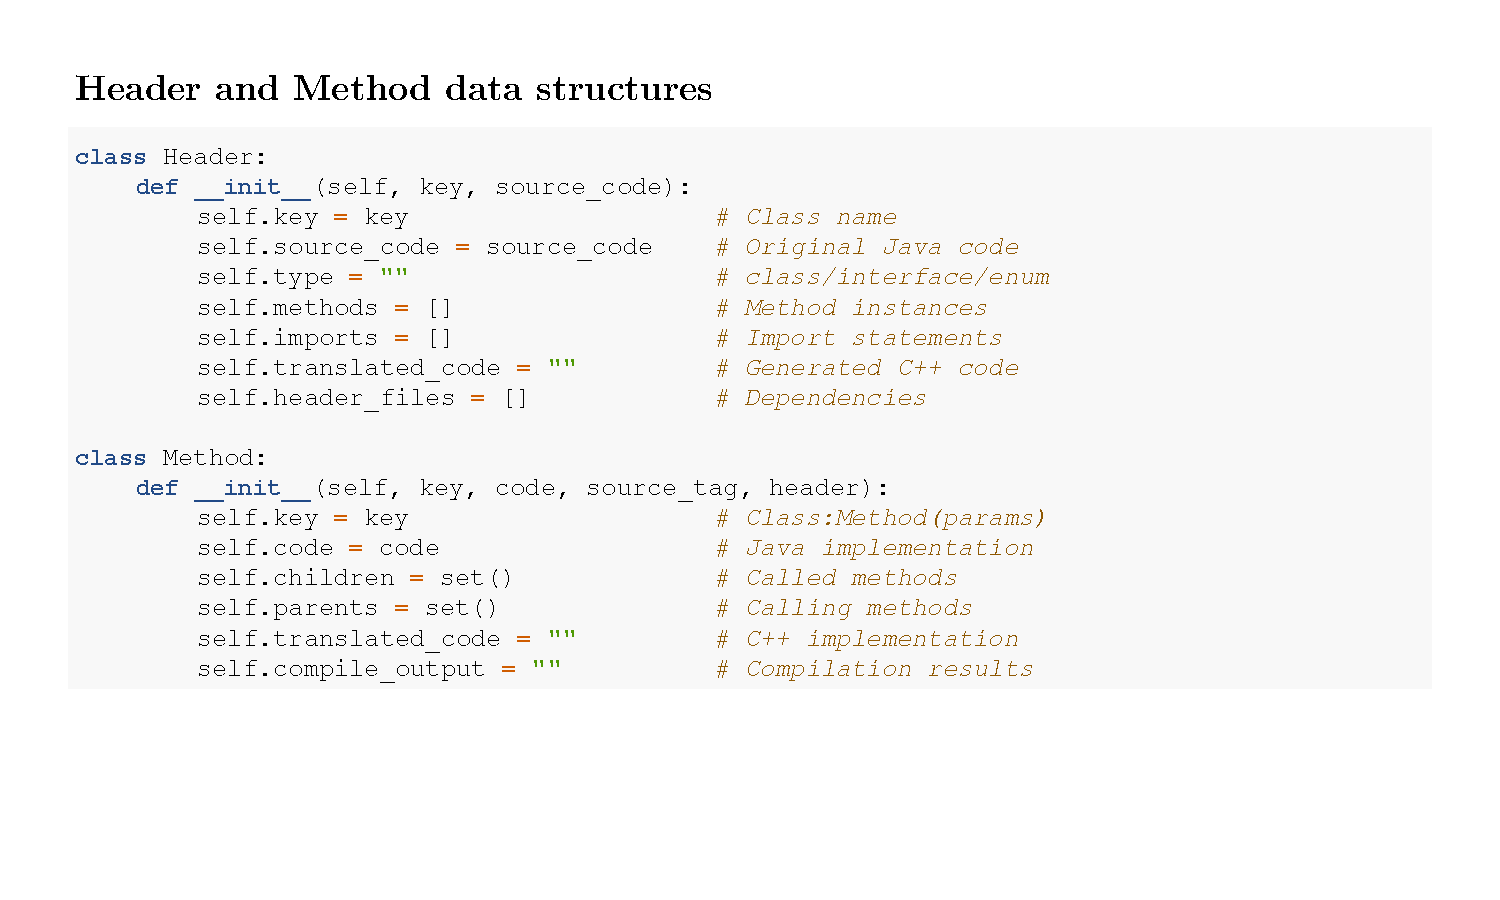
\includegraphics[width=\columnwidth]{code/fig3-5-header-method-data-structures.pdf}
\caption{Header and Method data structures}
\label{fig:data-structures}
\end{figure}

\subsection{Hierarchical Translation Engine}

\subsubsection{Basic process of translation}
\paragraph{Code splitting} Due to the fact that the scale of the project far exceeds the context limit of the large model, the code must be split in a reasonable and orderly manner to facilitate batch translation. We divide the nodes in the graph obtained in the previous section into two categories: one category records class-related information, including inheritance relationships, fields, various method declarations, etc.; the other category records the specific implementation information of methods. Our main translation objects are these two types of code fragments. For the translation from Java to C++, the former will generate C++ header files after analysis by the large model, and the latter will generate the implementation of C++ methods. 
\paragraph{Translation order}
Among the two types of nodes mentioned above, the head node is translated first. After that, all method nodes are topologically sorted according to their call relationships and then translated in sequence. The advantage of this order is that when translating the head node, the large model can focus on macro control and framework determination. When translating a certain method node next, the information of the head node to which the method node belongs and the information of previously translated nodes can serve as context to provide additional information. Using this method, the scale of translation can be expanded arbitrarily without worrying about the input length exceeding the model's limit, and it also reduces the occurrence of situations where the previously translated parts and the later translated parts are difficult to align.
\todo{TODO: Add a figure showing the translation order}

\subsubsection{Two-Phase Strategy}
While translating each node in graph(header or method), the translation engine implements a dual-phase approach:

\paragraph{Phase 1: Scheme Generation} In this phase, the large model understands and analyzes the code segment to be translated. For example, when translating "head node", the large model will determine the strategies for converting between language features (memory allocation, generics, standard library mapping, etc.) and type mapping. The figure \ref{fig:header-scheme-prompt} shows an example of a prompt for generating a header scheme.
\begin{figure}[h]
\centering
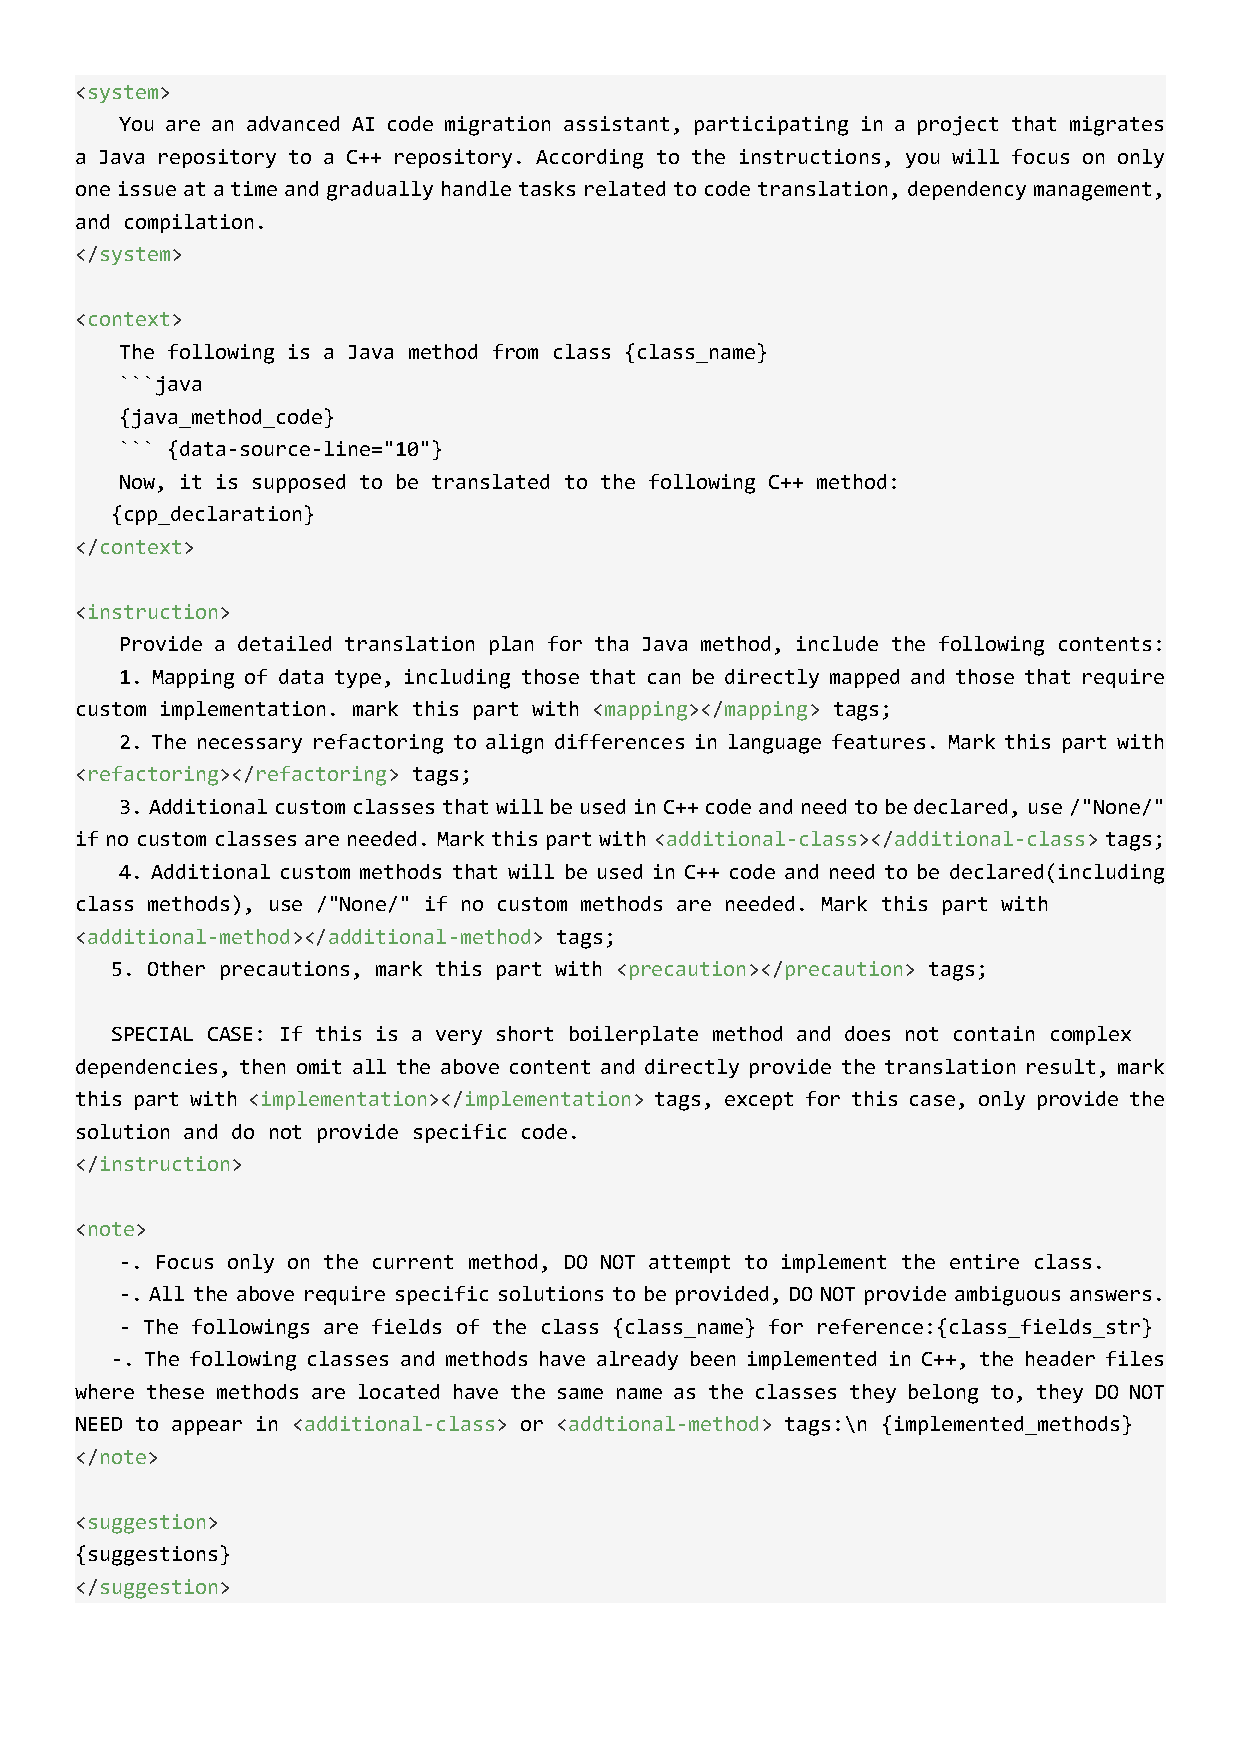
\includegraphics[width=\columnwidth]{figures/header-scheme-prompt.pdf}
\caption{header scheme generation prompt}
\label{fig:header-scheme-prompt}
\end{figure}

\paragraph{Phase 2: Code Generation}
At this stage, the generation of code in the target language officially begins, and by this time, the large model already has quite a rich context. \ref{fig:method-prompt} shows a example of method translation prompt, include:
\begin{itemize}
\item The transaltion scheme generated in Phase 1
\item The method signature declared in the head node
\item Other fields and methods related to the method
\end{itemize}

\begin{figure}[h]
\centering
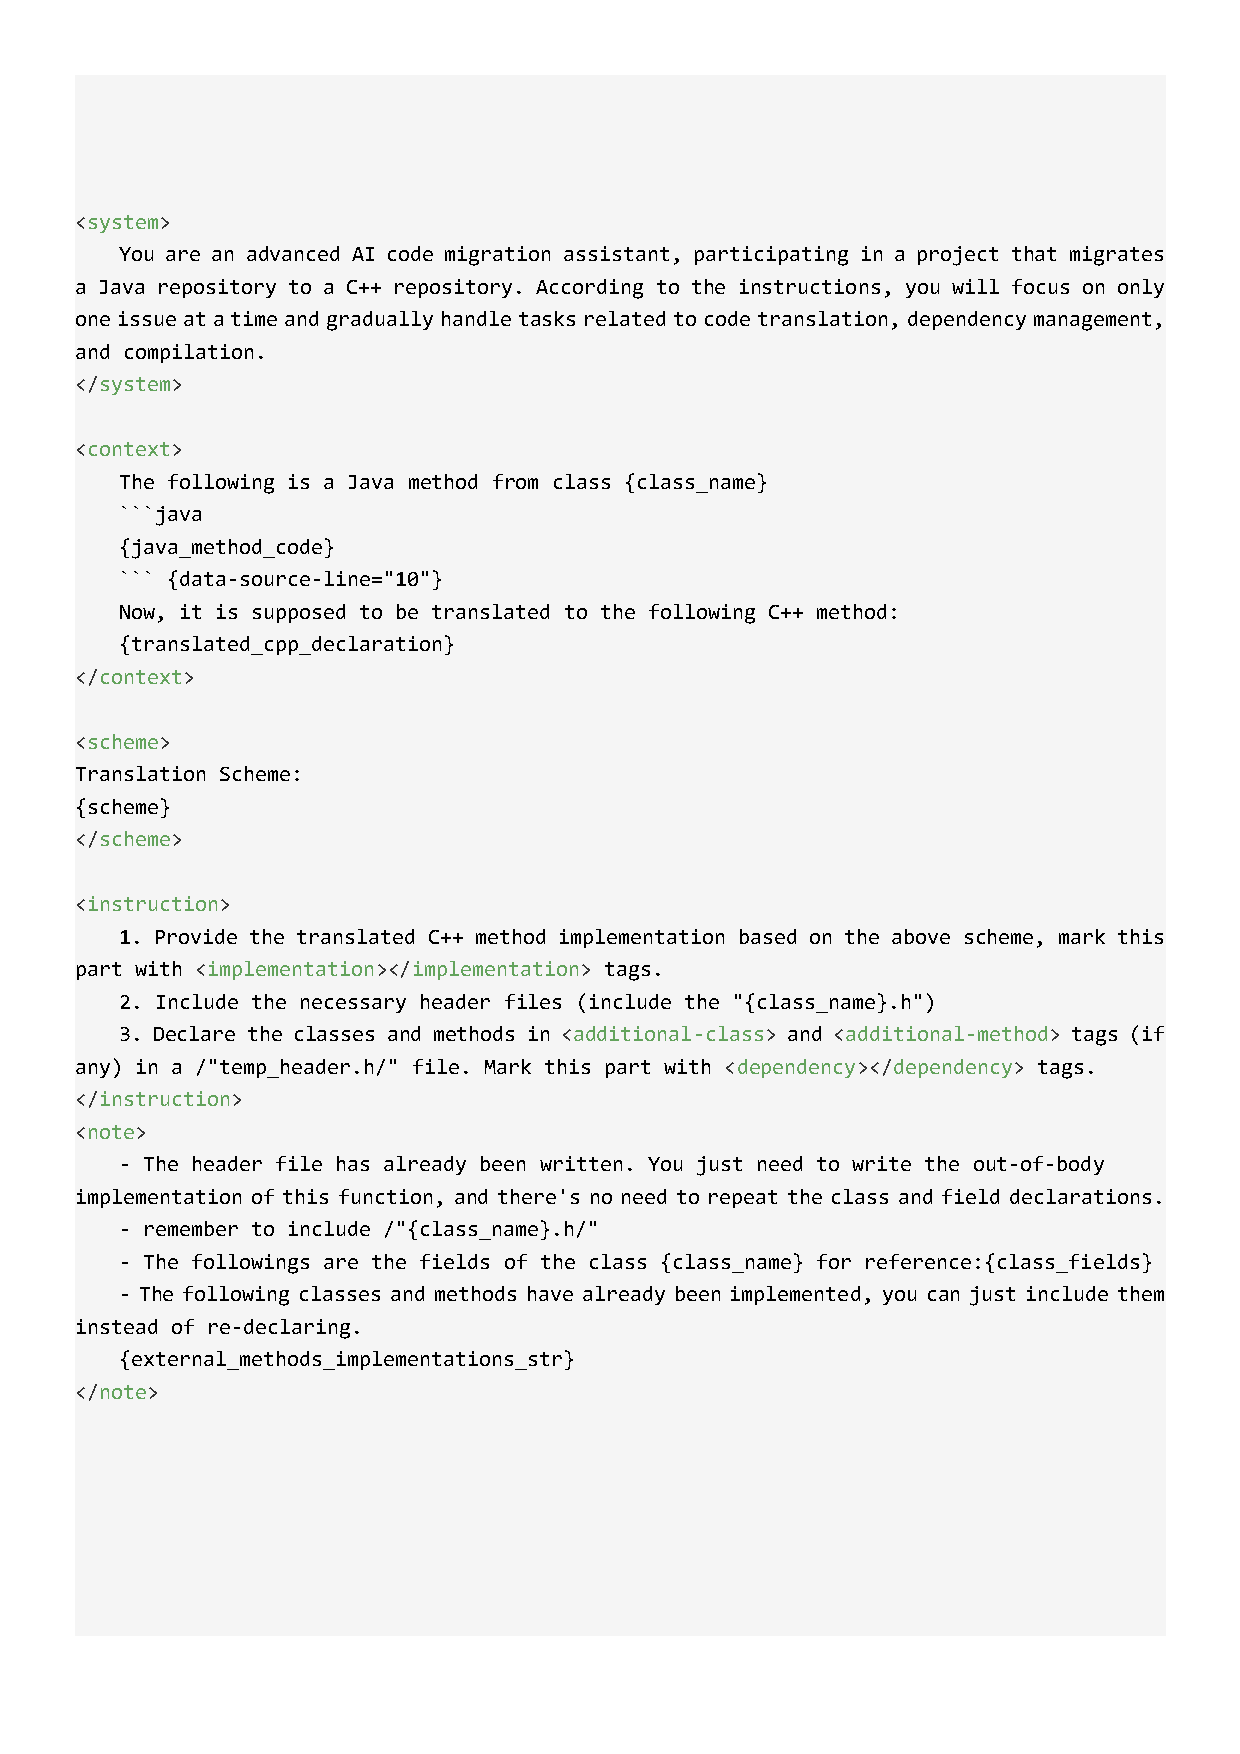
\includegraphics[width=\columnwidth]{figures/method-prompt.pdf}
\caption{method translation prompt}
\label{fig:method-prompt}
\end{figure}

\subsection{Autonomous Compilation Agent}

\subsubsection{Agent Architecture}
The compilation agent operates as an autonomous LLM-powered system with tool access:

\begin{itemize}
\item \textbf{Tool Suite}: File operations, compilation, error analysis
\item \textbf{Decision Engine}: LLM-based error diagnosis and fix planning
\item \textbf{State Management}: Conversation history and progress tracking
\end{itemize}

\subsubsection{Tool Interface}
The agent has access to four core tools:

\begin{figure}[h]
\centering
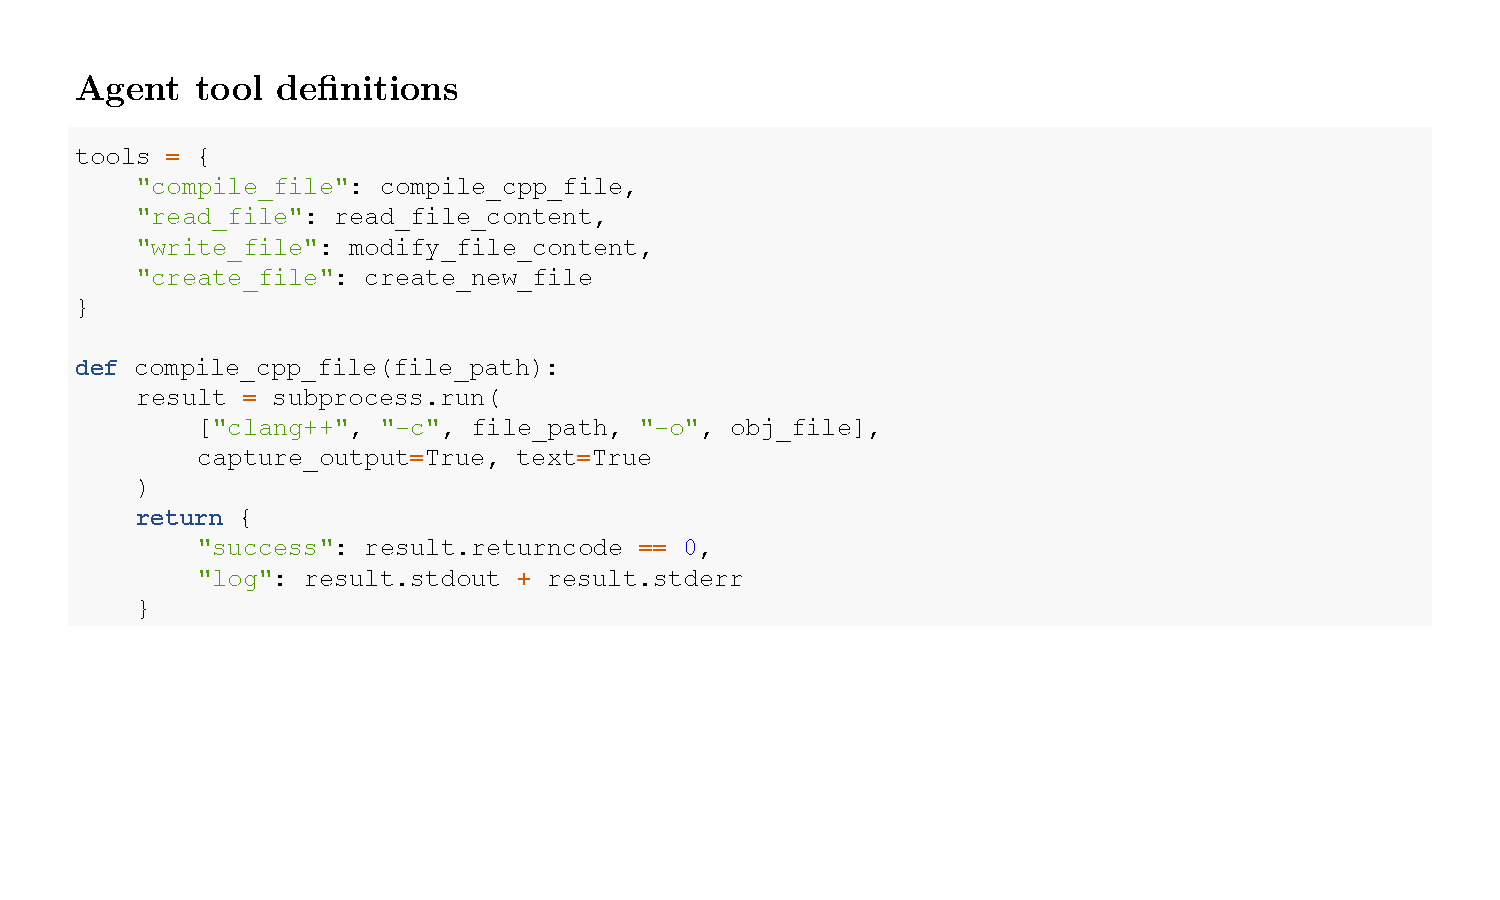
\includegraphics[width=\columnwidth]{code/fig3-4-agent-tool-interface.pdf}
\caption{Agent tool definitions}
\label{fig:agent-tools}
\end{figure}

\subsubsection{Error Resolution Strategy}
The agent follows a systematic approach to error resolution:

\begin{enumerate}
\item \textbf{Compilation}: Attempt to compile the target file
\item \textbf{Analysis}: Parse error messages and identify root causes
\item \textbf{Planning}: Generate fix strategies using LLM reasoning
\item \textbf{Execution}: Apply fixes through tool operations
\item \textbf{Validation}: Re-compile and verify resolution
\end{enumerate}

% \subsubsection{Intelligent Error Classification}
% The agent categorizes compilation errors and applies specific fix strategies:

% \begin{table}[h]
% \centering
% \small
% \begin{tabular}{ll}
% \toprule
% \textbf{Error Type} & \textbf{Fix Strategy} \\
% \midrule
% Missing includes & Add appropriate header files \\
% Type mismatches & Apply type conversions and templates \\
% Syntax errors & Fix brackets, semicolons, keywords \\
% Linker errors & Generate missing function implementations \\
% Namespace issues & Add proper namespace declarations \\
% \bottomrule
% \end{tabular}
% \caption{Error classification and corresponding fix strategies}
% \label{tab:error-strategies}
% \end{table}



This comprehensive implementation enables robust, scalable translation of Java projects to C++ while maintaining code quality and minimizing error propagation through the hierarchical approach and intelligent compilation repair mechanisms.